% UCL Thesis LaTeX Template
%  (c) Ian Kirker, 2014
% 
% This is a template/skeleton for PhD/MPhil/MRes theses.
%
% It uses a rather split-up file structure because this tends to
%  work well for large, complex documents.
% We suggest using one file per chapter, but you may wish to use more
%  or fewer separate files than that.
% We've also separated out various bits of configuration into their
%  own files, to keep everything neat.
% Note that the \input command just streams in whatever file you give
%  it, while the \include command adds a page break, and does some
%  extra organisation to make compilation faster. Note that you can't
%  use \include inside an \include-d file.
% We suggest using \input for settings and configuration files that
%  you always want to use, and \include for each section of content.
% If you do that, it also means you can use the \includeonly statement
%  to only compile up the section you're currently interested in.
% You might also want to put figures into their own files to be \input.

% For more information on \input and \include, see:
%  http://tex.stackexchange.com/questions/246/when-should-i-use-input-vs-include


% Formatting and binding rules for theses are here: 
%  https://www.ucl.ac.uk/students/exams-and-assessments/research-assessments/format-bind-and-submit-your-thesis-general-guidance

% This package goes first and foremost, because it checks all 
%  your syntax for mistakes and some old-fashioned LaTeX commands.
% Note that normally you should load your documentclass before 
%  packages, because some packages change behaviour based on
%  your document settings.
% Also, for those confused by the RequirePackage here vs usepackage
%  elsewhere, usepackage cannot be used before the documentclass
%  command, while RequirePackage can. That's the only functional
%  difference as far as I'm aware.
\RequirePackage[l2tabu, orthodox]{nag}


% ------ Main document class specification ------
% The draft option here prevents images being inserted,
%  and adds chunky black bars to boxes that are exceeding 
%  the page width (to show that they are).
% The oneside option can optionally be replaced by twoside if
%  you intend to print double-sided. Note that this is
%  *specifically permitted* by the UCL thesis formatting
%  guidelines.
%
% Valid options in terms of type are:
%  phd
%  mres
%  mphil
%\documentclass[12pt,phd,draft,a4paper,oneside]{ucl_thesis}
\documentclass[12pt,msc,a4paper,oneside]{ucl_thesis}


% Package configuration:
%  LaTeX uses "packages" to add extra commands and features.
%  There are quite a few useful ones, so we've put them in a 
%   separate file.
% -------- Packages --------

% This package just gives you a quick way to dump in some sample text.
% You can remove it -- it's just here for the examples.
\usepackage{blindtext}

% This package means empty pages (pages with no text) won't get stuff
%  like chapter names at the top of the page. It's mostly cosmetic.
\usepackage{emptypage}

% The graphicx package adds the \includegraphics command,
%  which is your basic command for adding a picture.
\usepackage{graphicx}

\graphicspath{
    {images}
}

% The float package improves LaTeX's handling of floats,
%  and also adds the option to *force* LaTeX to put the float
%  HERE, with the [H] option to the float environment.
\usepackage{float}

% The amsmath package enhances the various ways of including
%  maths, including adding the align environment for aligned
%  equations.
\usepackage{amsmath}

% for math symbol
\usepackage{ amssymb }

% Use these two packages together -- they define symbols
%  for e.g. units that you can use in both text and math mode.
\usepackage{gensymb}
\usepackage{textcomp}
% You may also want the units package for making little
%  fractions for unit specifications.
%\usepackage{units}


% The setspace package lets you use 1.5-sized or double line spacing.
\usepackage{setspace}
\setstretch{1.5}

% That just does body text -- if you want to expand *everything*,
%  including footnotes and tables, use this instead:
%\renewcommand{\baselinestretch}{1.5}


% PGFPlots is either a really clunky or really good way to add graphs
%  into your document, depending on your point of view.
% There's waaaaay too much information on using this to cover here,
%  so, you might want to start here:
%   http://pgfplots.sourceforge.net/
%  or here:
%   http://pgfplots.sourceforge.net/pgfplots.pdf
%\usepackage{pgfplots}
%\pgfplotsset{compat=1.3} % <- this fixed axis labels in the version I was using

% PGFPlotsTable can help you make tables a little more easily than
%  usual in LaTeX.
% If you're going to have to paste data in a lot, I'd suggest using it.
%  You might want to start with the manual, here:
%  http://pgfplots.sourceforge.net/pgfplotstable.pdf
%\usepackage{pgfplotstable}

% These settings are also recommended for using with pgfplotstable.
%\pgfplotstableset{
%	% these columns/<colname>/.style={<options>} things define a style
%	% which applies to <colname> only.
%	empty cells with={--}, % replace empty cells with '--'
%	every head row/.style={before row=\toprule,after row=\midrule},
%	every last row/.style={after row=\bottomrule}
%}


% The mhchem package provides chemistry formula typesetting commands
%  e.g. \ce{H2O}
%\usepackage[version=3]{mhchem}

% And the chemfig package gives a weird command for adding Lewis 
%  diagrams, for e.g. organic molecules
%\usepackage{chemfig}

% The linenumbers command from the lineno package adds line numbers
%  alongside your text that can be useful for discussing edits 
%  in drafts.
% Remove or comment out the command for proper versions.
%\usepackage[modulo]{lineno}
% \linenumbers 


% Alternatively, you can use the ifdraft package to let you add
%  commands that will only be used in draft versions
%\usepackage{ifdraft}

% For example, the following adds a watermark if the draft mode is on.
%\ifdraft{
%  \usepackage{draftwatermark}
%  \SetWatermarkText{\shortstack{\textsc{Draft Mode}\\ \strut \\ \strut \\ \strut}}
%  \SetWatermarkScale{0.5}
%  \SetWatermarkAngle{90}
%}


% The multirow package adds the option to make cells span 
%  rows in tables.
\usepackage{multirow}


% Subfig allows you to create figures within figures, to, for example,
%  make a single figure with 4 individually labeled and referenceable
%  sub-figures.
% It's quite fiddly to use, so check the documentation.
%\usepackage{subfig}

% The natbib package allows book-type citations commonly used in
%  longer works, and less commonly in science articles (IME).
% e.g. (Saucer et al., 1993) rather than [1]
% More details are here: http://merkel.zoneo.net/Latex/natbib.php
%\usepackage{natbib}

% The bibentry package (along with the \nobibliography* command)
%  allows putting full reference lines inline.
%  See: 
%   http://tex.stackexchange.com/questions/2905/how-can-i-list-references-from-bibtex-file-in-line-with-commentary
\usepackage{bibentry} 

% The isorot package allows you to put things sideways 
%  (or indeed, at any angle) on a page.
% This can be useful for wide graphs or other figures.
%\usepackage{isorot}

% The caption package adds more options for caption formatting.
% This set-up makes hanging labels, makes the caption text smaller
%  than the body text, and makes the label bold.
% Highly recommended.
\usepackage[format=hang,font=small,labelfont=bf]{caption}

% If you're getting into defining your own commands, you might want
%  to check out the etoolbox package -- it defines a few commands
%  that can make it easier to make commands robust.
\usepackage{etoolbox}

% The microtype package adds `micro-typographic extensions' which
% generally makes text more readable and hyphenation less likely.
\usepackage{microtype}

% for todo notes when writing essay
% usage: \todo{some notes...}
\usepackage{todonotes}



% Sets up links within your document, for e.g. contents page entries
%  and references, and also PDF metadata.
% You should edit this!
%%
%% This file uses the hyperref package to make your thesis have metadata embedded in the PDF, 
%%  and also adds links to be able to click on references and contents page entries to go to 
%%  the pages.
%%

% Some hacks are necessary to make bibentry and hyperref play nicely.
% See: http://tex.stackexchange.com/questions/65348/clash-between-bibentry-and-hyperref-with-bibstyle-elsart-harv
\usepackage{bibentry}
\makeatletter\let\saved@bibitem\@bibitem\makeatother
% \usepackage[hyphens]{url}
\usepackage[pdftex,hidelinks,breaklinks]{hyperref}
\makeatletter\let\@bibitem\saved@bibitem\makeatother
\makeatletter
\AtBeginDocument{
    \hypersetup{
        pdfsubject={Thesis Subject},
        pdfkeywords={Thesis Keywords},
        pdfauthor={Author},
        pdftitle={Title}
    }
}
\makeatother
    


% And then some settings in separate files.
\input{FloatSettings} % For things like figures and tables
\input{BibSettings}   % For bibliographies

% These control how many number sections your subsections will take
%    e.g. Section 2.3.1.5.6.3
%  and how many of those will get put into the contents pages.
\setcounter{secnumdepth}{3}
\setcounter{tocdepth}{3}


\begin{document}

\nobibliography*
% ^-- This is a dumb trick that works with the bibentry package to let
%  you put bibliography entries whereever you like.
% I used this to put references to papers a chapter's work was 
%  published in at the end of that chapter.
% For more information, see: http://stefaanlippens.net/bibentry

% If you haven't finished making your full BibTex file yet, you
%  might find this useful -- it'll just replace all your
%  citations with little superscript notes.
% Uncomment to use.
%\renewcommand{\cite}[1]{\emph{\textsuperscript{[#1]}}}

% At last, content! Remember filenames are case-sensitive and 
%  *must not* include spaces.
% I may change the way this is done in a future version, 
%  but given that some people needed it, if you need a different degree title 
%  (e.g. Master of Science, Master in Science, Master of Arts, etc)
%  uncomment the following 3 lines and set as appropriate (this *has* to be before \maketitle)
% \makeatletter
% \renewcommand {\@degree@string} {Master of Things}
% \makeatother

\title{Machine Learning for 2D Animation}
\author{Candidate No. QJTV4}  % receive an email saying thesis needs to be anonymous
\department{Department of Computer Science}

\maketitle
\makedeclaration

\begin{abstract} % 300 word limit
This preceding project researches and implements state-of-the-art (SOTA) methods in machine learning image-to-image translation for enhancing 2D animation development workflow. It tries to address the waterfall development problem by allowing artists to preview outcomes given initial creative inputs. Combining the task of frame interpolation, image colourization, sketch simplification, and super-resolution, this work indicates possible future directions and limitations for future iterations and further studies.
\end{abstract}

% Tobias says he don't read impact statement
% \begin{impactstatement}
% 	In the 2D animation industry, the process of creating 2D animation consists of a number of steps, some of which could be labour-intensive and often constitute up to 50\% of the budget. The industry is falling behind when it comes to creative tools in 2D animation. Currently, the lead artist gives front-loaded creative inputs followed by intensive labour tasks over which he has little control. We want the artist to have an accurate preview of what might be in the final product. Contrasting to traditional approaches, our proposed workflow is designed around the capabilities of the artists, allowing them to take a shot from start to finish with creative control along the way. The final tool-set will allow one animator to complete work that typically requires five animators to do.
% \end{impactstatement}

\begin{acknowledgements}
I very much appreciate Dr Tobias Ritschel, Professor of Computer Graphics at University College London, for supervising this project. This work is also in collaboration with NoGhost, a real-time creative animation studio based in London. Especially, I would also like to extend my sincere thanks to Jack Straw and Luke Gibbard from NoGhost for their continued support throughout the project.
\end{acknowledgements}



\setcounter{tocdepth}{2} 
% Setting this higher means you get contents entries for
%  more minor section headers.

\tableofcontents

\listoffigures




% I have no table
% \listoftables


\chapter{Introductory}
\label{chapterlabel1}
\section{Background}

\subsection{2D Animation Pipeline}
2D animation is a manipulation of objects such that they appear as moving objects. It usually consists of a sequence of frames drawn by hand with computer-assisted technologies. The process of creating 2D animation consists of some labour-intensive tasks that depend on early-stage decisions. Once the development moves on to the next stage, it is very difficult or comes with a large cost to go back and change something that was not well thought out in the concept stage. This is known as the \textit{waterfall development model}\footnote{This is more of a term used in software development, but I think it is suitable to use here. See \url{https://en.wikipedia.org/wiki/Waterfall\_model} for more information.}. By improving this development process, we can save time and money, and have greater opportunities to improve the quality and quantity of work done, this could have a huge effect on the industry as a whole. In the following paragraphs, I will introduce (1) the current process for creating 2D animation;  (2) the proposed workflow; (3) the role of this master project and thesis. 


\subsubsection{Current Process}
In the current 2D animation creation process, the lead artist gives front-loaded creative input followed by labour-intensive tasks over that he has little control. I have listed the main stages of the existing 2D animation workflow as follows:

\begin{enumerate}
    \item \textbf{Key Poses / Layout} Setting up major actions and placement.
    \item \textbf{Roughs / Inbetweening} Assign timing and frame distribution.
    \item \textbf{Cleanup / Inking} Clean sketches, add styling and motion effects.
    \item \textbf{Coloring / Mattes} Coloring, add shadows and highlights.
\end{enumerate}

\begin{figure}
    \centering
    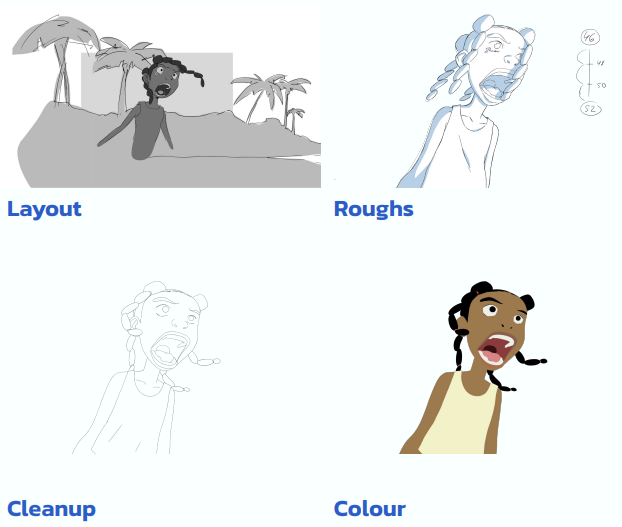
\includegraphics[width=0.75\textwidth]{images/introduction/stages.png}
    \caption{Sample frame for 4 stages of the workflow, including Layout, Roughs, Cleanup and Colour.} 
    \todo[inline]{Separate images and discuss what is happening in individual step, with more samples. (Ask NoGhost for more layout samples)}
    \label{fig:stages}
\end{figure}

We can see that the major actions and character placement are fixed after the first stage, there are only very rough sketches that define the starting and ending points of a transition (known as \textit{keyframes}), which is difficult to work with. \todo{show some samples of this} We want the lead artist to get an accurate preview of what might be the final product and offers potential creative options. This is going to enhance and speed up the process of creating 2D animation.

\subsubsection{Proposed System}

\begin{figure}
    \centering
    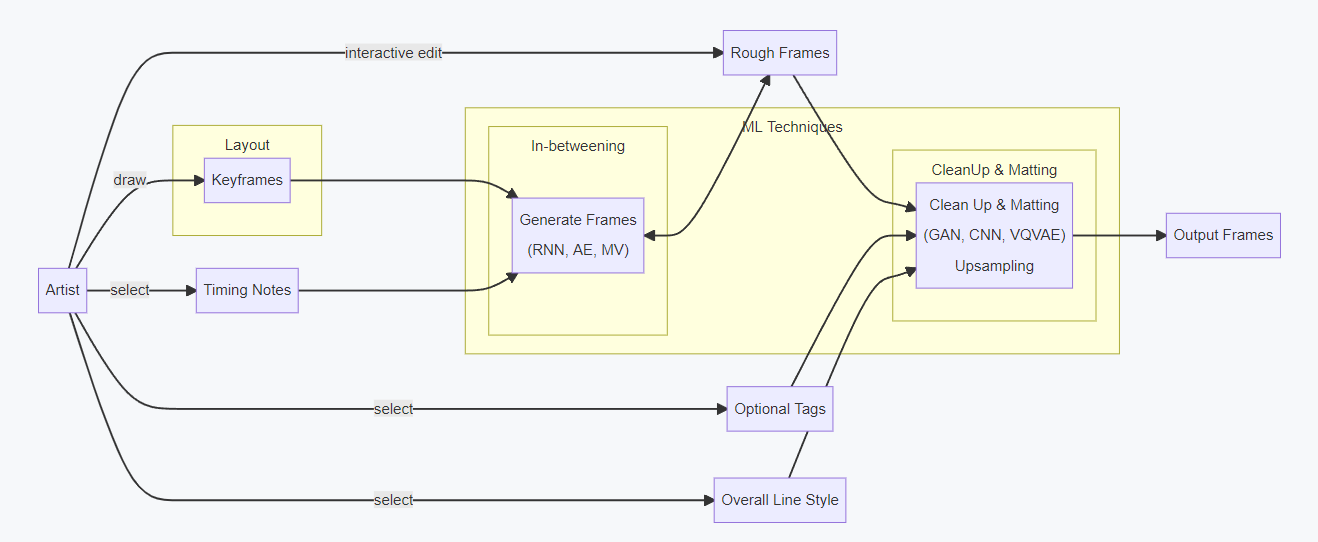
\includegraphics[width=1\textwidth]{images/introduction/proposed_workflow.png}
    \caption{Overview of proposed final workflow for the artist. The artist will produce a number of rough frames, with timing and style information. They will be feed into multiple machine learning (ML) pipelines to generate a preview of the final animation.} 
    \label{fig:proposed_worflow}
\end{figure}

In the proposed system, the artist will produce a number of rough keyframes with timing and style information. These frames will go through 4 ML pipelines, each consist of a separate task: (1) cleaning up the rough sketches; (2) colouring; (3) frame interpolation (increase fps) and (4) upscaling (super-resolution).

The role of this master project and thesis is to (1) research each task, (2) develop a prototype model, (3) generate a proof-of-concept report and suggest future development direction.


\section{General Approach}
\subsection{Image-to-Image Translation}
All four tasks fall into the field of Image-to-Image translation (I2I), which is a sub-field in Computer Vision. I2I refers to the task of transforming images from one domain to another so that they have the styles or characteristics from another domain. It has been gaining popularity in recent years due to its wide range of applications in computer vision problems such as image restoration, super-resolution, segmentation and pose-estimation. The scope of this project falls into two-domain, supervised I2I\cite{pangImagetoImageTranslationMethods2021}. Most recent research on I2I uses deep convolutional neural networks to learn a mapping function between and source and target domain. Pix2pix\cite{isolaImagetoImageTranslationConditional2018} first successfully apply deep convolutional conditional GAN to solve a wide range of I2I problems. However, Pix2pix itself suffers from a number of issues. For example, training might be unstable and error-prone as resolution increases\cite{wangHighResolutionImageSynthesis2018}; and unable to capture complex scene structure\cite{tangMultiChannelAttentionSelection2019}. Thus we will not directly apply it in our tasks, however, most models are either inspired by or follow the same architecture as Pix2pix.

\subsection{Pretraining}
Many researchers found that in computer vision tasks, it is generally useful to first pre-train the model with a large amount of data and then finetune to downstream tasks\cite{baoBEiTBERTPreTraining2021, weiMaskedFeaturePrediction2021, newellHowUsefulSelfSupervised2020}. This is especially suitable in the context of this master project because the amount of data provided is a subset of all available data\cite{newellHowUsefulSelfSupervised2020}.

Pretraining can be seen as a form of weight initialization, and weight initialization is important when training neural networks. In the early days, some researchers initialize their neural network's weight to all zeros, and they soon find that this results in the \textit{symmetry problem} (see appendix \ref{app:ml:sym}) which makes the network harder to learn. Some researchers proposed random initialization, which works well in some cases, but if you are unlucky, you can run into initialization that is either too large or too small, which will result in exploding and vanishing gradient problems respectively (see appendix \ref{app:ml:van_grad}). An popular alternative is Xavier initialization\cite{glorotUnderstandingDifficultyTraining2010} (see appendix \ref{app:ml:van_grad:weight_init}).


\begin{figure}
    \centering
    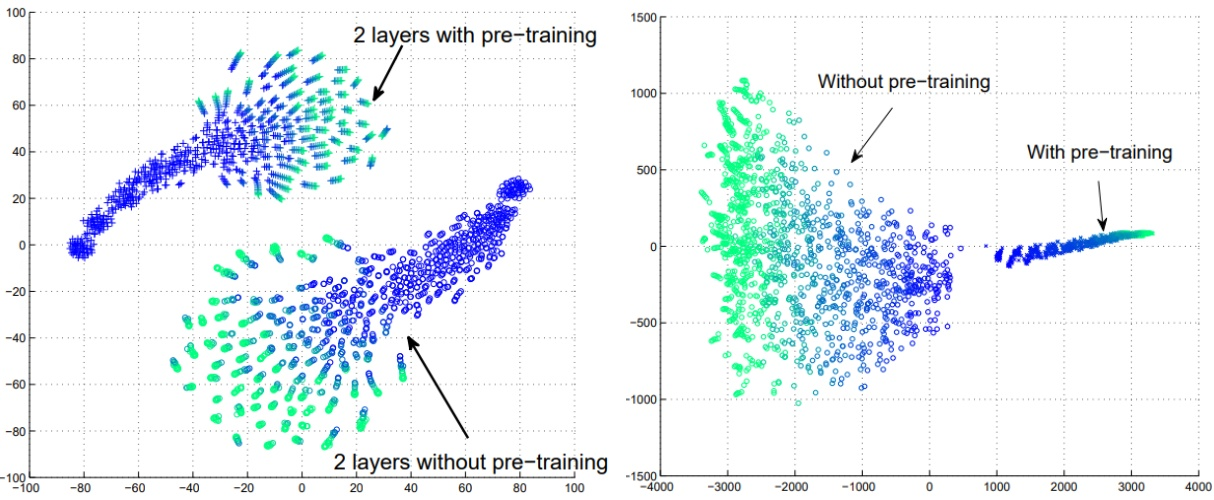
\includegraphics[width=1\textwidth]{images/introduction/pretrain_vis.jpg}
    \caption{Visualization of training progress of simple 2-layer networks. Left is visualized with t-SNE (see appendix \ref{app:stat:tsne}) and right is visualized with ISOMAP (see appendix \ref{app:stat:isomap}) Color from blue to cyan indicates a progression in training iterations. 50 of them are with pretraining (crosses) and another 50 of them are without pretraining (circles). We can observe that training with pretraining is generally faster, and more stable than training without pretraining.\cite{erhanWhyDoesUnsupervised}} 
    \label{fig:pretrain_tsne}
\end{figure}

Although Xavier can improve initialization mathematically, the network will likely start far from the optimum. Pretraining on the other hand, when applied on a similar task, allow the model to start closer to the optimum, improving convergence time by reusing patterns learnt and improving model robustness\cite{hendrycksUsingPreTrainingCan2019} (see figure \ref{fig:pretrain_robustness}).


\begin{figure}
    \centering
    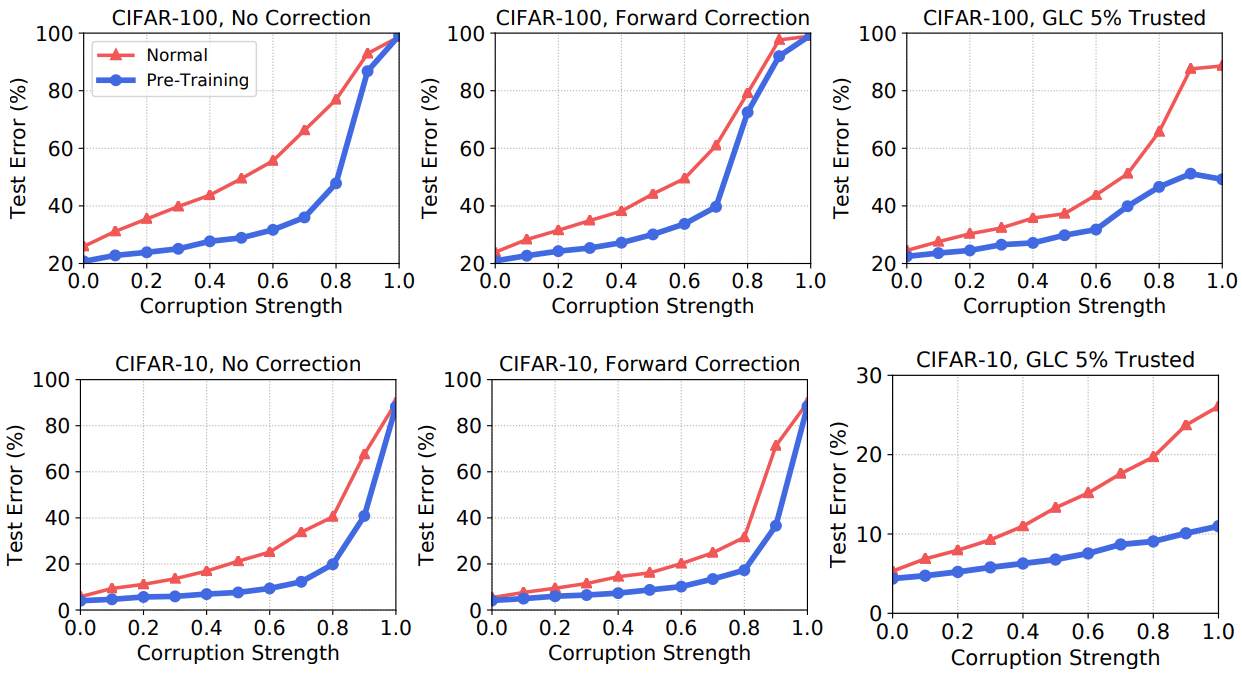
\includegraphics[width=0.75\textwidth]{images/introduction/pretrain_robustness.png}
    \caption{Classification error rate for a typical Wide ResNet\cite{zagoruykoWideResidualNetworks2017} on the CIFAR-10 and CIFAR-100 dataset with varying \textit{corruption strength} on the label during training. \textit{Corruption strength} refers to the probability of a training label is incorrect. We can observe that pretraining always outperforms training from scratch.} 
    \label{fig:pretrain_robustness}
\end{figure}

However, it is worth noting that pretraining does not necessarily improve result quality when a large training dataset is provided. Recent work showed that the benefits of pretraining diminish exponentially with increasing training data available. When sufficient data is provided, pretraining merely speeds up training on vision tasks\cite{heRethinkingImageNetPretraining2018}. Some studies even suggest that the pre-trained model performs worse because it is difficult for weights to completely abandon previously learned patterns, although it is theoretically possible\cite{el-noubyAreLargescaleDatasets2021}. 

Besides finetuning for downstream tasks, it can also be used as a feature extractor to enhance the network's capability for a variety of vision tasks. A popular choice is pre-trained vision transformer\cite{dosovitskiyImageWorth16x162021}, which is an attention-based network that achieved comparative results with SOTA convolutional neural network while requiring less computation. Some studies even directly used pre-trained feature extractors for vision classification tasks and achieved modest accuracy\cite{awaisCanPretrainedConvolutional2020}.


\subsection{Preprocessing}

\begin{figure}
    \centering
    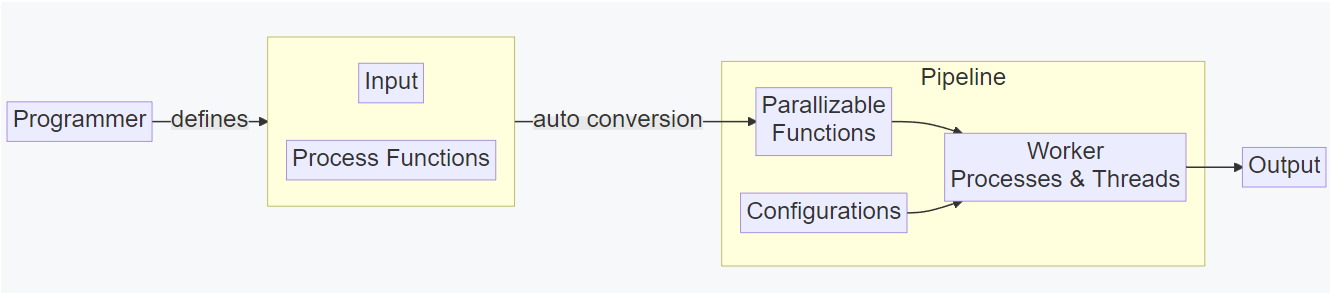
\includegraphics[width=1.0\textwidth]{images/introduction/preprocess_pipeline.png}
    \caption{Overview of Preprocessing pipeline. In a typical use case, the programmer will first define a set of input and processing functions, feeds them into the pipeline and runs it. The pipeline will automatically convert the inputs into parallelizable functions and split them evenly across processes and threads for efficient processing, and finally produce the processed output.} 
    \label{fig:preprocess_pipeline}
\end{figure}

There is a need for processing a large number of image files into a specific format, size and directory for this master project. To achieve this, I developed a small generalized multiprocessing \& multithreading pipeline in Python\cite{WelcomePythonOrg}. Together with pre-built modular processing functions, it provides a set of flexible and maintainable procedures for processing (see figure \ref{fig:preprocess_pipeline}).




%Pretraining + finetuning + feature content loss + WGAN-GP, cGAN + U-Net

% Tobias says not relevant
% \subsection{Diffusion Model}
% Recently, diffusion model has been gaining popularity and shown comparative benchmarks on various computer vision tasks\cite{sahariaPaletteImagetoImageDiffusion2022, dhariwalDiffusionModelsBeat2021}. Although it is relatively new and has not been studied extensively and I did not apply them directly. I will briefly introduce them in case of interest in the future because it is highly potential.

% Diffusion model can be traced back to 2015 when researchers proposed a generative machine learning approach that is highly flexible and computationally tractable\cite{sohl-dicksteinDeepUnsupervisedLearning2015}. The idea is to develop a forward diffusion process that systematically and slowly erases the structure in the data, and then learn a backward diffusion process that recovers it. However, it did not attract much attention. Later, a stochastic differential equation that transforms complex data distribution to a known prior distribution based on the diffusion process was presented\cite{songScoreBasedGenerativeModeling2021}. It showed that the diffusion model can produce comparative performance in certain image generation tasks like inpainting by slowly introducing Gaussian noise into the forward diffusion process, and then learning its reverse process. A denoising diffusion model\cite{hoDenoisingDiffusionProbabilistic2020} also showed that it is capable of generating high-quality images.

% \todo[inline]{TODO: introduce diffusion model researches}

% \section{Evaluation Methods}
%mostly by eye, we can compute the PSNR and SSIM, but, generally, the eye is enough.
%Some stuff about things.\cite{example-citation} Some more things. 

%Inline citation: \bibentry{example-citation}

% This just dumps some pseudo-Latin in so you can see some text in place.
%\blindtext

\chapter{Preliminaries}
\label{chapterlabel2}

\section{U-Net}

\section{Pix2pix}

\section{cGAN}

\section{pixelshuffle}

\section{resnext}


\chapter{Colorization}
\label{chapterlabel3}

\section{Approaches \& Methods}
\section{Benefits \& Limitations}
\section{Design \& Implementation}
\section{Results \& Analysis}
% This just dumps some pseudolatin in so you can see some text in place.
\blindtext

\chapter{Sketch Simplification}
\label{chapterlabel4}
\section{Approaches \& Methods}
\section{Benefits \& Limitations}
\section{Design \& Implementation}
\section{Results \& Analysis}
% This just dumps some pseudolatin in so you can see some text in place.
\blindtext

% Tobias says he would like me to focus on two areas only
% \chapter{Super Resolution}
\label{chapterlabel5}
\section{Approaches \& Methods}
\section{Benefits \& Limitations}
\section{Design \& Implementation}
\section{Results \& Analysis}
% This just dumps some pseudolatin in so you can see some text in place.
% \blindtext

% \chapter{Frame Interpolation}
\label{chapterlabel6}
\section{Approaches \& Methods}
\section{Benefits \& Limitations}
\section{Design \& Implementation}
\section{Results \& Analysis}
% This just dumps some pseudolatin in so you can see some text in place.
\blindtext

\chapter{Future \& Directions}
\label{chapterlabel7}

\section{State of Tasks}
One of the main purposes of this thesis is to provide a development review of tasks. In a nutshell, the amount of research and progress can be ranked from low to high: Colourization $<$ Sketch Simplification $<$ Frame Interpolation $\leq$ Super Resolution. Super resolution is a long-standing task as it is applicable to any videos. Frame interpolation can be used to increase frame rate of any low-resolution videos therefore it also has a considerable amount of interest in reseaarch industry. Both tasks are popular research areas in recent years, with little finetuning effort, it is possible to generate accurate outputs with real-time performance. Sketch simplification on the other hand, is 2D animation specific, therefore there are comparatively less research interest. It can be viewed as a task to remove noise, however, the definition of noise can vary and result in less effort devoted to our region of interest. Nevertheless, it is a relatively simple task if we can obtain high-quality training samples. Colourization seems to be a field with mature solutions. However, solutions in traditional grayscale image colourization task do not apply directly to 2D anime-style sketches. This is because anime-style sketches have less information and less well-defined objective function, making it the most challenging and time-consuming task out of all.

\section{Next Steps}

The most critical action item for NoGhost is to create appropriate datasets. For most machine learning tasks, the dataset is much more important than the model architecture or training procedure. Learning from noisy labels severely degrades the performance and generalization capability of any model. Especially in the context of 2D animation since many subtasks are relatively straightforward. Although research that tries to handle datasets with noise with robust learning methods such as regularization, loss adjustments, sample selection and noise adaptation layers\cite{songLearningNoisyLabels2022}, it remains a challenging task and we should avoid them in the production environment.

In terms of research, sketch simplification should be prioritized. This is because it is the first step in the pipeline, a fast and high-quality output can provide a solid foundation for subsequent tasks. Unlike colourization, it is also a more well-defined task with a clear objective, and the optimization techniques proposed in the previous sections are relatively easy to implement, making it suitable for new machine learning researchers to learn about image-to-image translation. The follow-up task would be to tackle the colourization task. As the most complicated task, it requires intensive experiments, by starting early, we can better understand the limitation of current SOTA models and set out the timeline and compromises needed for a working prototype.

In term of software engineering, we should set up the whole pipeline as early as possible, even if some of the models are not producing satisfactory results. So that we can set expectations on how much more optimizations are needed for a real-time system, and get a better grip on the capability of the whole system.

Lastly, detailed future directions for a specific task are written at the end of the corresponding chapter. Researchers are strongly advised to check them out before proceed with further experiments.

% Although some fields remained under-explored, existing research is able to solve most problems and is more than enough for the purpose of generating previews for lead artists. 

% This just dumps some pseudolatin in so you can see some text in place.
% \blindtext

\chapter{General Conclusions}
\label{chapterlabel8}

To summarise, modern 2D animation consists of a sequence of complex and time-consuming tasks, automating these procedures is a challenging task. This master project investigates the possibility of automating such workflow to generate creative previews. We split the proposed automation system into four individual image-to-image translation tasks, researched independently and conducted several experiments that reflected positively. Collectively, we found that recent machine learning models are capable of generating high-quality samples on each task. While there can be technical difficulties while integrating the parts, We can conclude that the proposed system is a feasible solution to give artists an accurate preview with near real-time performance.

% This just dumps some pseudo-Latin in so you can see some text in place.
% \blindtext

\phantomsection
\addcontentsline{toc}{chapter}{Appendices}

% The \appendix command resets the chapter counter, and changes the chapter numbering scheme to capital letters.
%\chapter{Appendices}
\appendix
\chapter{Machine Learning}
\label{app:ml}

\section{Vanishing Gradient}
\label{app:ml:van_grad}
When training neural network using back-propagation, each of the network layer's weights receives an update by computing a partial derivative given its next layer's partial derivative using chain rule. The problem is the weights of the layer can be small i.e. (0, 1], this is especially the case if you use a traditional activation such as hyperbolic tangent function which clips the output to range of (0, 1]. When back-propagating, the gradient is going to be multiplied by a value in range of (0,1] many times. This means that the gradient is getting smaller and smaller as we back-propagate (thus the term \textit{vanishing}), and when it finally reaches beginning layers of the network, the gradient can be too small for them to perform any meaningful update, thus preventing the layers from learning. For a deep network such as GAN, vanishing gradient is more likely to occur since the gradient need to be back-propagated through both discriminator and generator. A closely related problem is exploding gradient problem, which the gradient increases instead of decreases. There have been multiple proposed solutions to this problem. I will briefly describe them below:

\begin{itemize}
    \item \textbf{Batch Normalization} is a widely adopted method for solving both exploding and vanishing gradient problem. It reduces the internal covariate shift\cite{ioffeBatchNormalizationAccelerating2015a} and reduces local optimum by smoothing the optimization landscape\cite{santurkarHowDoesBatch2018}.
    \item \textbf{Residual Network} is the most effective way to solve the vanishing gradient problem. It refers to a network architecture that implements skip/residual connection. It creates shortcuts for gradient to flow through without diminishing/exploding.
    \item \textbf{Activation Function} if used appropriately, can reduce the chance of vanishing gradient. For example, ReLU suffers less because gradient does not saturate on the active path (i.e. positive values)\cite{glorotDeepSparseRectifier2011}.
    \item \textbf{Weight Initialization}\label{app:ml:van_grad:weight_init} could be helpful to reduce weight initialization by adjusting them to follow a certain distribution. For example, Xavier\cite{glorotUnderstandingDifficultyTraining2010} initialize weights such that mean of the activations are zeros, and the variance of the activations stay the same across every layer. In other words, weights of a layer $l$ are randomly sampled from a Gaussian/normal distribution with mean $\mu = 0$ and variance $\sigma^2=\frac{1}{n_{l-1}}$, where $n_{l-1}$ is the number of neurons in the previous layer, and bias are initialized with zeros.
\end{itemize}

\section{Mode Collapse}
\label{app:ml:mode_col}
A well trained model would produce a wide variety of outputs, however, it may stuck in a special kind of local minimum. Let's consider a scenario: our generator found a small subset of outputs that produces an especially plausible for the discriminator, we call the current version of generator $\mathcal{G}_1$ and discriminator $\mathcal{D}_1$. As training continues, the discriminator would learn to reject this subset and result in $\mathcal{D}_2$.  However, the generator evolves to $\mathcal{G}_2$ as well and learned to produce another small subset of plausible output for $\mathcal{D}_2$. Now in order to learn to reject $\mathcal{G}_2$'s output, the discriminator may not evolves to a new $\mathcal{D}_3$, instead, it may fallback to $\mathcal{D}_1$, because it can probably reject $\mathcal{G}_2$'s output as well. Then the generator and discriminator just cycling through these two versions and not making any real progress. This form of failure is called mode collapse.

\section{Non-Convergence}
\label{app:ml:non_conv}
As the generator improves over time, the discriminator performance will get worse, because it can no longer tell a difference between real and fake output. The discriminator will just make random guess. Now the feedback from the discriminator is meaningless and can degrade generator performance, when the generator performance degrades, the discriminator can again provide meaningful feedback, and the loop continues. This means that when training GAN, it is hard to determine when to stop, as it does not necessarily reduced to a stable state.

\section{Symmetry Problem}
\label{app:ml:sym}
In the context of weight initialization, symmetry problem is an argument for weights should not be initialized as same value. This is because if the weights are equal, then its gradient will be equal, and the weights are going to be updated by the same amount. If these weights are attached to the same neuron, it will theoretically remain the same throughout training, and therefore its capability will decrease.

\section{Knowledge Distillation}
\label{app:ml:kd}
While large models such as very deep neural network can have large capacity, it may not be fully utilized. This means that we can potentially reduce the size of the model while achieve similar results. This process is called knowledge distillation.

\section{Weight Clipping}
\label{app:ml:weight_clip}
Weight clipping is to enforce gradient in a network to have a specific minimum or/and maximum if they exceed a certain range. It can be used to prevent exploding gradient, but generally, this does not fix the real underlying problem. More commonly, it is used in Wasserstein GAN to enforce the \textit{dual representation theorem} constraint so that Wasserstein distance can be computed efficiently. Let $W$ be any $m\times l$ matrix, $c=\max|W|$, and $||\cdot||_s$ be operator norm of the matrix (the element with largest singular value, in other words, the maximum absolute value of its eigenvalues), we have:
$$
||W||_s^2\leq c^2ml^2
$$
by clipping all entries of $W$ within some interval $[-c, c]$. Thus we can bound $||W||_s$ and restrict the discriminator to have a bounded Lipschitz norm.

\section{Gradient Penalty}
\label{app:ml:grad_pen}
Gradient penalty is used in Wasserstein GAN to enforce the \textit{dual representation theorem} constraint so that Wasserstein distance can be computed efficiently. It is a loss for the discriminator in GAN in the form of:
$$
\mathbb{E}_{x \sim \hat{\mu}}\left[\left(\|\nabla D(x)\|_{2}-a\right)^{2}\right]
$$
where $\hat{\mu}$ is a fixed distribution, and $a$ is the targeted value. During training, the discriminator will attempt to minimize the difference between $\nabla D(x)$ and $a$, bringing all its gradient close to $a$, and thus restricts the discriminator to have bounded Lipschitz norm.

\section{Skip/Residual Connection}
\label{app:ml:res_conn}
Residual connection is a technique used to allow an neural network block to \textit{modify} the  input instead of \textit{transform} the input. Additionally, the output holds a reference to the input which allows the gradient to shortcut the previous block directly. There is empirical evidence showing deep neural network built with this technique is easier to optimize. Essentially, applying such technique is to change a function $f$ from $f(x)$ to $f(x)+x$. Figure \ref{fig:res_conn} further illustrate such technique.

\begin{figure}
    \centering
    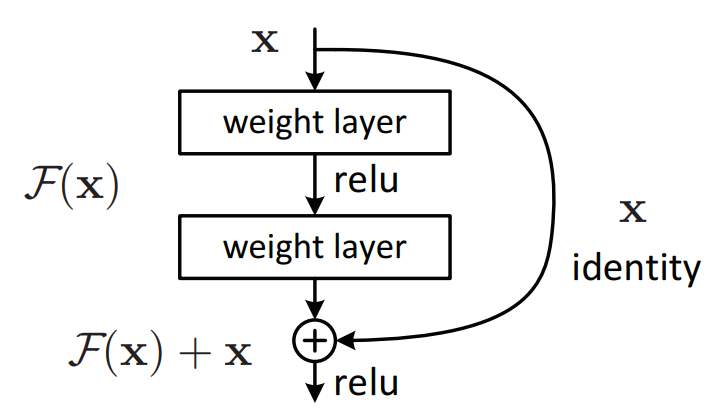
\includegraphics[width=0.45\textwidth]{images/preliminary/res_conn.png}
    \caption{Residual Connection block. The input of the block is element-wise added to the output of the block, creating a shortcut for the gradient to flow through.\cite{heDeepResidualLearning2015a}}
    \label{fig:res_conn}
\end{figure}

\section{Pre-Activation}
\label{app:ml:pre_act}

\section{Pixel Shuffle}
\label{app:ml:pix_shuf}

\begin{figure}
    \centering
    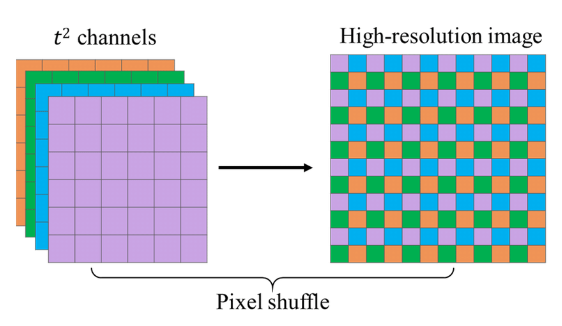
\includegraphics[width=0.45\textwidth]{images/appendix/pixel_shuffle.png}
    \caption{Illustration of the pixel shuffle operation. $t^2$ channels of features are combined in an interleaving manner, effectively resulting in a sub-pixel}
    \label{fig:pixel_shuffle}
\end{figure}

Pixels Shuffle is a function often used in super-resolution models to implement efficient sub-pixel convolution. It convolutes the image using $t^2$ channels and combines features in different channels, interleaving each other. 

Note that this is a different operation than transpose convolution. Transpose convolution increases the size of the feature map by convolution with stride, while pixels shuffle increases resolution by flattening multiple feature maps into one. 



\chapter{Statistics}
\label{app:stat}

\section{tSNE}
\label{app:stat:tsne}
TSNE stands for t-distributed stochastic neighbour embedding. It is a probabilistic-based method for visualizing high dimensional data by assigning data points in different dimensions onto different regions on a 2 or 3-dimensional grid. Specifically, this assignment method is called Stochastic Neighbor Embedding\cite{hintonStochasticNeighborEmbedding2002}. A pleasant feature of this method is that it preserves neighbour identities, which means similar features will be placed closer together.

\section{ISOMAP}
\label{app:stat:isomap}


\chapter{Miscellanous}

\section{NoGhost Dataset}
\label{app:misc:noghostdata}
The NoGhost dataset is provided in GoogleDrive\footnote{Link with restricted access: \url{https://drive.google.com/drive/folders/1C0BppKuJMm29BdusdknqcNxJWGy__Kok?usp=sharing}, please contact NoGhost for accessing the dataset.}. The structure of the dataset is shown in figure \ref{fig:noghost_dataset_structure}. Each innermost folder contains  frames of a character in that particular shot of a specific stage of development.
\begin{figure}
    \centering
    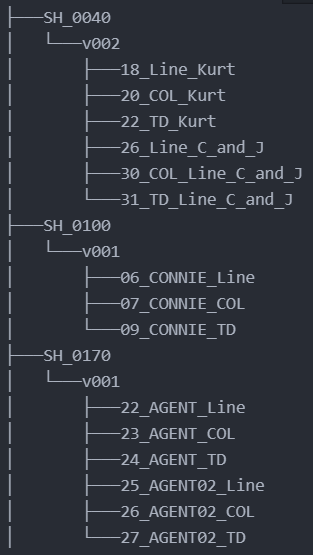
\includegraphics[width=0.35\textwidth]{images/appendix/noghost_dataset_structure.png}
    \caption{Subset of the folder structure of NoGhost's Dataset. The upper level is the shot folder, follow by version number and image folders, denoting different stages of development. Line: cleaned sketches; COL: colourized images; TD: uncleaned sketches}
    \label{fig:noghost_dataset_structure}
\end{figure}

\section{Image Hashing Algorithms}
\label{app:misc:image_hashing}
An image hash algorithm converts an image into a sequence of bytes. Ideally, it should: (1) produce an identical/similar hash for similar images; (2) particular strong resistance against noises such as salt and pepper, gaussian smoothing, and colour adjustment. (3) reasonably robust against the change of brightness, contrast, gamma correction, watermark, scaling, and jpeg compression, (3) optionally robust against transformation such as rotation and skew.

\subsection{Average Hashing}
This hash is robust against scale/aspect ratio, brightness/contrast, and colour (not too much). It is also very efficient to compute.
\begin{enumerate}
    \item \textbf{Reduce colour}, converts the image to grayscale.
    \item \textbf{Reduce size}, scales the image down to $8\times8$ (for 64 bits hash).
    \item \textbf{Generate hash}, set $1$ if the number in the $8\times8$ hash is more than its average value, else $0$.
\end{enumerate}

\subsection{Median Hashing}
Same as Average Hashing, except that it uses median instead of average. Performance is similar to Average Hashing.

\subsection{Perceptive Hashing}
The algorithm is similar to Average Hashing but uses discrete cosine transform to compare frequency instead of colour values. This hash outperforms the average hashing algorithm in almost aspects, in particular, it generates almost no false positives/negatives. However, it takes twice the time needed for the average hash algorithms.
\begin{enumerate}
    \item \textbf{Reduce colour}, converts the image to grayscale.
    \item \textbf{Reduce size}, scales the image down to $4*8 \times 4*8$ (for 64 bits hash).
    \item \textbf{Generate frequencies}, apply Discrete Cosine Transform (DCT) to generate frequency information, per row then per column, then crop the top-left ($8\times8$) corner which contains the high frequencies value.
    \item \textbf{Generate hash}, set $1$ if the number in the $8\times8$ hash is more than its median (not average) value, else $0$.
\end{enumerate}

\subsection{Block Hashing}
The image is divided into blocks and generates $1$ or $0$ for each block. These $1$s and $0$s are sequentially concatenated to form a binary hash number.

\subsection{Difference Hashing}
This algorithm generates very few false positives compared to Average Hashing and runs as fast.
\begin{enumerate}
    \item \textbf{Reduce colour}, converts the image to grayscale.
    \item \textbf{Reduce size}, scales the image down to $9\times8$ (for 64 bits hash).
    \item \textbf{Generate hash}, set $1$ if the number is more than its right pixels, else $0$
\end{enumerate}

\subsection{Wavelet Hashing}
Similar to perceptive hashing, but uses Discrete Wavelet Transformation (DWT) which is another form of frequency representation. The key advantage when compared to DCT is that it captures both frequency and location information\cite{DiscreteWaveletTransform2022}. 




% \chapter{Another Appendix About Things}
% \label{appendixlabel2}
% (things)

% \chapter{Colophon}
% \label{appendixlabel3}
% \textit{This is a description of the tools you used to make your thesis. It helps people make future documents, reminds them, and looks good.}

% \textit{(example)} This document was set in the Times Roman typeface using \LaTeX\ and Bib\TeX , composed with a text editor. 
 % description of the document, e.g. type faces, TeX used TeXmaker, packages and things used for figures. Like a computational details section.
% e.g. http://tex.stackexchange.com/questions/63468/what-is-best-way-to-mention-that-a-document-has-been-typeset-with-tex#63503

% Side note:
%http://tex.stackexchange.com/questions/1319/showcase-of-beautiful-typography-done-in-tex-friends

% You could separate these out into different files if you have
%  particularly large appendices.

% Actually generates your bibliography. The fact that \include is 
% the last thing before this ensures that it is on a clear page.
\bibliography{example}

% All done. \o/
\end{document}
